\documentclass[english]{article}

\usepackage[latin9]{inputenc}
\usepackage[letterpaper]{geometry}
\geometry{verbose,tmargin=1in,bmargin=1in,lmargin=1in,rmargin=1in}
\usepackage{amsmath}
\usepackage{amssymb}
\usepackage{tikz}
\usepackage{algpseudocode}
\usepackage{booktabs}

\usepackage{verbatim}
\usepackage{tkz-berge}
\usetikzlibrary{automata,positioning,arrows,shapes,petri,topaths}

\tikzstyle{dir}=[->, very thick]
\tikzstyle{circ}=[draw, circle, very thick]

\title{CIS 511 Homework 5}
\author{Stephen Phillips, Dagaen Golomb}
\date{April 8, 2015}


\begin{document}
\maketitle
\subsection*{Problem 1}
The NP-Completeness proof for SUBSET-SUM works because the input is encoded in log($n$) bits, so
solving the problem takes time exponential in the number of bits. Since complexity is measured
against the size of the input, this places SUBSET-SUM $\in$ NP.

However, for UNARY-SSUM, each number occupies length equal to its value. Therefore, we can convert
each number into binary which can be done in polynomial time via successive division by two and
checking any remainder (which becomes the next significant digit). This runs in polynomial time.
We do this for each number. Now, we have the classic SUBSET-SUM problem. We can solve this in a
brute-force manner by simulating the non-deterministic TM.

This simulation takes time exponential
in the length of the [created] input, which is log($n$) of the original input. Therefore, this
runs in time polynomial ($O(e^{log(n)}) = O(n)$) of the original input. Thus, UNARY-SSUM $\in$ P.

\subsection*{Problem 2}
\subsection*{Part a}
We know that $CNF_2 = \{\langle \phi \rangle \mid \phi \textrm{ is a satisfiable CNF formula with each 
variable appears at most 2 times}\}$ is in $P$ since we can make an algorithm for it.

\begin{algorithmic}
\Function{$M$}{$\phi$}
  \State Check that all variables $x_i$ appear at most twice as 
  \State Create $\psi$, a modifiable copy of $\phi$
  \State Create bit vector $b$ for the final assignment
  \ForAll{$i \in \{1, \ldots, n\}$}
    \If{There is one clause left}
      \State Accept
    \ElsIf{There is one variable left}
      \If{Clauses $x_i$ and $\bar{x_i}$ both are in $\phi$}
        \State Reject
      \Else
        \State Accept
      \EndIf
    \ElsIf{the literal $x_i$ appears once}
      \State $\psi \leftarrow \psi(x_i=1)$ (and simplify $\psi$)
    \ElsIf{the literal $\bar{x_i}$ appears once}
      \State $\psi \leftarrow \psi(x_i=0)$
    \ElsIf{the literal $x_i$ appears twice}
      \State $\psi \leftarrow \psi(x_i=1)$
    \ElsIf{the literal $bar{x_i}$ appears twice}
      \State $\psi \leftarrow \psi(x_i=0)$
    \Else
      \State Combine the clauses with $x_i$ and $\bar{x_i}$ in $\psi$ by creating a new clause with all the
              other literals in the two clauses together
    \EndIf
  \EndFor
\EndFunction 
\end{algorithmic}

We need to show that this works, so we analyze each case in the if else chain in the loop. We show
that each branch either makes the problem smaller, or solves the problem.
\begin{itemize}
\item If there is only one clause, we can set any literal in the clause to true and we have satisfied the problem,
        so we are done.
\item If there is one variable $x$ left, since we know each variable only appears twice, it is unsatisfiable if and 
        only if the clauses left are $x$ and $\bar{x}$, so we accept accordingly.
\item If a literal $x$ only appears once in the formula, we can just it to true and get rid of the clause that the
        the literal is in. Similarly, if the literal $\bar{x}$ is in only once, we can just set it to false to get
        rid of the clause
\item If the literal $x$ appears twice in the formula (or equivalently $\bar{x}$), then we can like before just set
        the literal to the appropriate value and get rid of the clauses that it occupies.
\item The tricky case - if $x$ and $\bar{x}$ both appear in different clauses. Note however that:
        \[ (x + a)(\bar{x} + b) \iff \bar{x}a + xb + ab \iff a + b \]
      Since we can choose $x$ accordingly. So it is satisifiable if and only if $a + b$ is true, so we combine
      the clauses and continue.
\end{itemize}

Since we reduce the problem by at least one variable each time, with simple boolean formula manipulations
in each step, we can run this in polynomial time in the number of clauses and variables. Therefore, this is
in $P$.

\subsection*{Part b}
We show that $CNF_3 = \{\langle \phi \rangle \mid \phi \textrm{ is a satisfiable CNF formula with each 
variable appears at most 3 times}\}$ is NP-Complete. We show how to change an instance of $3SAT$ to
an instance in $CNF_3$.

Given a $3SAT$ we can increase the number of variables to make sure that no one variable shows more than 3 times. 
Let us say a variable $x$ shows up in $k$ clauses. Then we create new variables $y_1,\ldots,y_k$. We create a `chain'
of implications:
\[y_1 \implies y_2 \implies y_3 \implies \ldots \implies y_n \implies y_1\]
This means all these variables must have the same value. In CNF form, using $x \implies y \iff (\bar{x} + y)$,
this would be 
\[(\bar{y_1} + y_2)(\bar{y_2} + y_3) \ldots (\bar{y_n} + y_1)\]
Then for each clause that $x$ is in, we use one of the $y_i$ variables. Now each of the $y_i$ variables appears
twice in the `chain' of implications, and once in the actual clauses, meaning it appears a total of 3 times. 

We illustrate with an example, using the simple example with only the variable $x$:
\begin{align*}
& (x + a_1 + b_1)(x + a_2 + b_2)(\bar{x} + a_2 + b_2)(\bar{x} + a_4 + b_4) \\
\end{align*}

This becomes with these new rules:
\begin{align*}
& (\bar{y_1} + y_2)(\bar{y_2} + y_3)(\bar{y_3} + y_4)(\bar{y_4} + y_1) \\
& (y_1 + a_1 + b_1)(y_2 + a_2 + b_2)(\bar{y_3} + a_2 + b_2)(\bar{y_4} + a_4 + b_4) \\
\end{align*}

Now we need to make sure this is still a polynomial time transformation. Say there are $n$ variables and $m$
clauses. In the worse case, a variable appears in every clause. This means we add $m$ variables to the equation,
and $m$ clauses for the `chain' of implications. If this happens for each variable we get $mn$ new clauses, and
$mn$ new variables, given $O(mn)$ sized problem, which is just a quadratic blow up in this size of the formula,
and therefore still a polynomial time transformation. Therefore if we can solve $CNF_3$ we can solve $3SAT$ which
we know to be NP-complete. Since checking a boolean formula is in NP since we can use the assignment as a 
certificate, this is NP-complete

\subsection*{Problem 3}
Let the Mine Consistency Problem (MCP) be as defined in the problem:\\
$\{G : G \text{ has a satisfiable assignment of mines}\}$.

This is clearly in P: given a graph with mines and numbers, it is easy to check if this it is a
consistent and accurate labeling. Now we will show MCP $\in$ NP by reducing MCP to SAT. This will
show MCP is at least as hard as SAT and hence in NP.

Let us define a variable $x_{ijk}$ that, for each $0 \le k \le 8$, represents if the cell at row $i$
and column $j$ has value $k$. Note in this notation we are using $k = 0$ to represent the presence
of a mine.

The reduction works as follows. For all $i,j,k$, we create a conjunction
($x_{ijk} \cdot \bar{x_{ijk'}}$)
for each $k' \neq k$. This enforces that each cell cannot be assigned two different values. We also 
produce the disjunction ($x_{ij0} + x_{ij1} + ... + x_{ij8}$) for each $i,j$ pair. This means each cell 
must be assigned some value. These expressions in total enforce each cell to have exactly one value.

Next we will enforce the rules of Minesweeper. For each $x_{ijk}$ we enumerate all positional
combinations of $k$ mines around the number and build expressions to match them. Note for $x_{ij0}$
we will not place any restrictions since the expressions for the numbered cells will enforce the
game rules. For example, for $k = 1$ for some $i,j$, we create the conjunction
($x_{ij1} \cdot x_{(i+1)j1} \cdot \bar{x_{(i+1)j1}} \cdot ...$) with the remaining adjacent cells
being not literals. This is an example of a valid configuration for a cell marked as 1 with only
a mine in the position below it. Note that these expressions are similar for edge nodes with the
omission of cells that do not exist (making the construction even easier). Note that although
combinations in general grow combinatorially, we are only dealing with specific combinations which
are a constant number of expressions each. Therefore, this operation still only takes constant time
for each cell. Finally, we "or" each combination together to allow any combination of $k$ mines
around the cell.

We now assert that the above Boolean formula is satisfiable $\iff$ there is a consistent mine
placement.

\begin{itemize}
	\item $\implies$
	Given a satisfiable assignment to the above formula, pick the true $x_{ij0}$'s for each $i,j$.
	By construction, no other $x_{ijk}$ value is true, and each adjacent numbered cell must account
	for this mine. Therefore, this mine is placed in a valid position and consistent with the game
	rules. Since this holds for each mine, this is a consistent mine placement.
	\item $\Longleftarrow$
	Given a consistent mine placement, set each mine position's $x_{ij0}$ to true and set the literals
	for other values of $k$ to false. For each numbered cell set the corresponding $x_{ijk}$ to true
	(if it is marked with $k$) and set the other literals over $i,j$ to false. Now each cell has
	a distinct assignment so the first part of the construction is true. Also, since this is a
	consistent marking, the second expression is true by construction as well. Therefore, the
	conjunction of these two are true and the formula is satisfiable.
\end{itemize}

\subsection*{Problem 4}
If $P = NP$, then there exists a polynomial time decider $D$ for $SAT$ runs in polynomial time. From this we can
create a new machine $M$ that finds the assignment of the variables. The idea is that we assign true or false to
each of the variables in order, and use $D$ to determine if it is a valid assignment. If there are multiple
assignments we just pick the one that works in order of the variables.

\begin{algorithmic}
\Function{$M$}{$\phi$}
	\State Create $\psi$, a modifiable copy of $\phi$
	\State Create bit vector $b$ for the final assignment
	\ForAll{$i \in \{1, \ldots, n\}$}
		\State Set $\psi' \leftarrow \psi(x_i=1)$
		\If{$D(\psi')$ accepts}
			\State $\psi \leftarrow \psi'$
			\State $b_i \leftarrow 1$ 
		\Else
			\State $\psi \leftarrow \psi(x_i=0)$
			\State $b_i \leftarrow 0$ 
		\EndIf
	\EndFor
	\State Output $b$
\EndFunction 
\end{algorithmic}

In words, we greedily go through the variables assigning them. We initially assign each variable $x_i$ to 1, and use
$D$ to check if that assignment is feasbile. If it is, then there must be a valid assignment where $x_i$ is 1, and if
not $x_i$ must be 0. So we assign $x_i$ appropriately. Then we update the formula to reflect this choice, and
continue appropriately.

Now we show this runs in polynomial time. Let $n$ be the number of variables, and $m$ be the number of clauses in the
original formula. On each iteration of the outer loop, we update the formula, which takes $O(m)$ time, and we run
the decider $D$, which runs polynomial time for some polynomial $p(n+m)$. There are $n$ iterations of the loop, so in
total this takes $O(nm p(n+m))$ time, which is still a polynomial.

\subsection*{Problem 5}

\subsection*{Problem 6}
We want to, given a CNF formula $\phi$, construct an NFA that accepts all nonaccepting configurations of $\phi$.
The idea is we create a sub-NFA for each clause that accepts if and only if the clause is false. To illustrate,
we use a simple formula over 4 variables $\phi(x_1,x_2,x_3,x_4) = (x_2 + x_3 + \bar{x_4})$

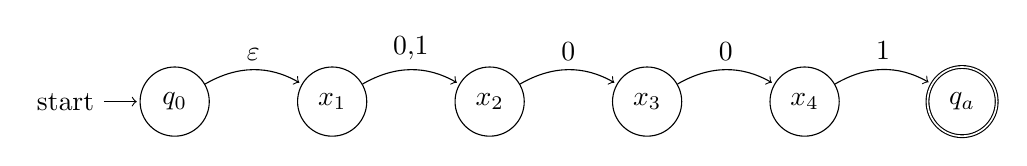
\begin{tikzpicture}[shorten >=1pt,node distance=2cm,on grid,auto] 
   \node[state,initial]   (q_0000)   {$q_0$}; 
   \node[state]           (q_0001) [right=of q_0000] {$x_1$}; 
   \node[state]           (q_0010) [right=of q_0001] {$x_2$}; 
   \node[state]           (q_0011) [right=of q_0010] {$x_3$};
   \node[state]           (q_0100) [right=of q_0011] {$x_4$};
   \node[state,accepting] (q_0101) [right=of q_0100] {$q_a$};
    \path[->] 
    (q_0000) edge[bend left] node {$\varepsilon$}  (q_0001)
    (q_0001) edge[bend left] node {0,1} (q_0010)
    (q_0010) edge[bend left] node {0} (q_0011)
    (q_0011) edge[bend left] node {0} (q_0100)
    (q_0100) edge[bend left] node {1} (q_0101);
\end{tikzpicture}

This takes in as input the bit string representing the assignment of all the variables. Each of the successive nodes
represents the variables, and they transition to the next node on values that would allow the clause to reject.
Notice that since $x_1$ does not appear in the clause, it can take whatever value it wants. So this accepts
the non-satisfying strings ${0,1}001$. 

We can generalize this to more clauses, by making the initial state have $\varepsilon$-transitions 
to a chain for each clause, constructed in the exact same way as the above example. That would
give, with $m$ variables and $c$ clauses, $cm$ nodes. The transition function would take then
$O(cm)$ space to create. This means it can be created in $O(cm)$, or polynomial, time.
This new NFA would accept on any rejecting input since it only takes one failing clause to make the formula
reject. 

If this formula has no accepting input, this NFA would reduce to one that accepts $\{0,1\}^*$, or:

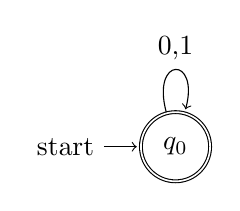
\begin{tikzpicture}[shorten >=1pt,node distance=2cm,on grid,auto] 
   \node[state,initial,accepting] (q_0000)   {$q_0$}; 
    \path[->] 
    (q_0000) edge[loop above] node {0,1} (q_0000);
\end{tikzpicture}

Therefore if we could reduce this NFA in polynomial, we would be able to solve SAT in polynomial time. In other
words we just reduced SAT to minimizing an NFA. Therefore if $P\neq NP$ then there is no polynomial time solution
for this.

\subsection*{Problem 7}
We want to show that the problem of designating directions to edges of an undirected graph $G$ so that a given subset
$C$ will have all nodes in it have either indegree 0 or outdegree 0, and all other nodes have indegree at least one
is NP-complete. We reduce SAT to this. And example of the mapping is show for the formula
$\phi(x_1,x_2,x_3,x_4) = (x_1 + \bar{x_2} + x_3)(\bar{x_1} + x_2 + x_4)(\bar{x_2} + \bar{x_3} + \bar{x_4})$


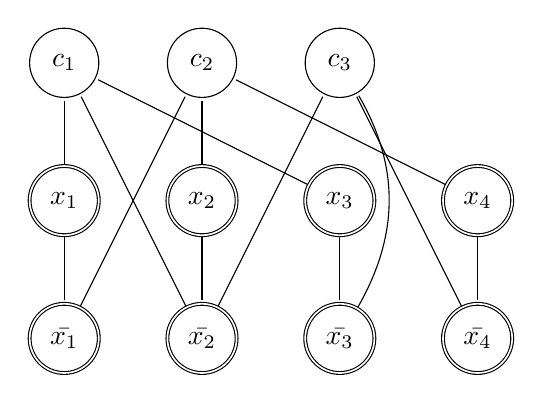
\begin{tikzpicture}[shorten >=1pt,node distance=1.75cm,on grid,auto] 
   \node[state]           (c_1)                 {$c_1$}; 
   \node[state]           (c_2)  [right=of c_1] {$c_2$}; 
   \node[state]           (c_3)  [right=of c_2] {$c_3$}; 
   \node[state,accepting] (x_1)  [below=of c_1] {$x_1$};
   \node[state,accepting] (x_2)  [right=of x_1] {$x_2$};
   \node[state,accepting] (x_3)  [right=of x_2] {$x_3$};
   \node[state,accepting] (x_4)  [right=of x_3] {$x_4$};
   \node[state,accepting] (x_1b) [below=of x_1] {$\bar{x_1}$};
   \node[state,accepting] (x_2b) [below=of x_2] {$\bar{x_2}$};
   \node[state,accepting] (x_3b) [below=of x_3] {$\bar{x_3}$};
   \node[state,accepting] (x_4b) [below=of x_4] {$\bar{x_4}$};
    \path[-] 
    (x_1)  edge             node {} (x_1b)
           edge             node {} (c_1)
    (x_1b) edge             node {} (c_2)
    (x_2)  edge             node {} (x_2b)
           edge             node {} (c_2)
    (x_2b) edge             node {} (c_1)
           edge             node {} (c_3)
    (x_3)  edge             node {} (x_3b)
           edge             node {} (c_1)
    (x_3b) edge[bend right] node {} (c_3)
    (x_4)  edge             node {} (x_4b)
           edge             node {} (c_2)
    (x_4b) edge             node {} (c_3);
\end{tikzpicture}

The highlighted nodes are the ones in $C$. 

We want to create such a graph for any SAT formula $\phi$. So in words the procedure is for every variable $x_i$,
create nodes $x_i$ and $\bar{x_i}$, and for every clause $c_j$ create a node $c_j$. Connect the node $x_i$
(or $\bar{x_i}$) to node $c_j$ if the variable $x_i$ (or $\bar{x_i}$) is in the clause $c_j$. Also create an edge
between nodes $x_i$ and $\bar{x_i}$. Place all the nodes $x_i$ and $\bar{x_i}$ into $C$. 

This graph has a solution the the direction problem if and only if the formula $\phi$ has a solution. If the
formula $\phi$ has a solution, select the true literals $x_i$/$\bar{x_i}$ as the `all outdegree' or 0 indegree nodes
in $C$, and the complement pair as the `all indegree' or 0 outdegree ones. Since only the pairs of literal nodes
$x_i$/$\bar{x_i}$ are connected in $C$, this does not lead to an inconsistency. If this is the satisfying assignment
then we should have at least one edge into each clause node $c_j$. Similarly, if we have such an assignment of edge
directions, we can reconstruct the satisfying assignment, since only one in each of the pairs of literal nodes
$x_i$/$\bar{x_i}$ has `all outdegree' we can set those literals to true, and we know by the direction assignment
that every clause will have one corresponding true literal inside it. Therefore, this graph has a solution to the
problem if and only if the the formula has a satisfying assignment. 


\end{document}

